\section{Motivation}
\begin{frame}
    \frametitle{Outline}
    \tableofcontents[currentsection]
\end{frame}

\begin{frame}
    \frametitle{Motivation}

    Consider the following plant structure
    \begin{figure}
        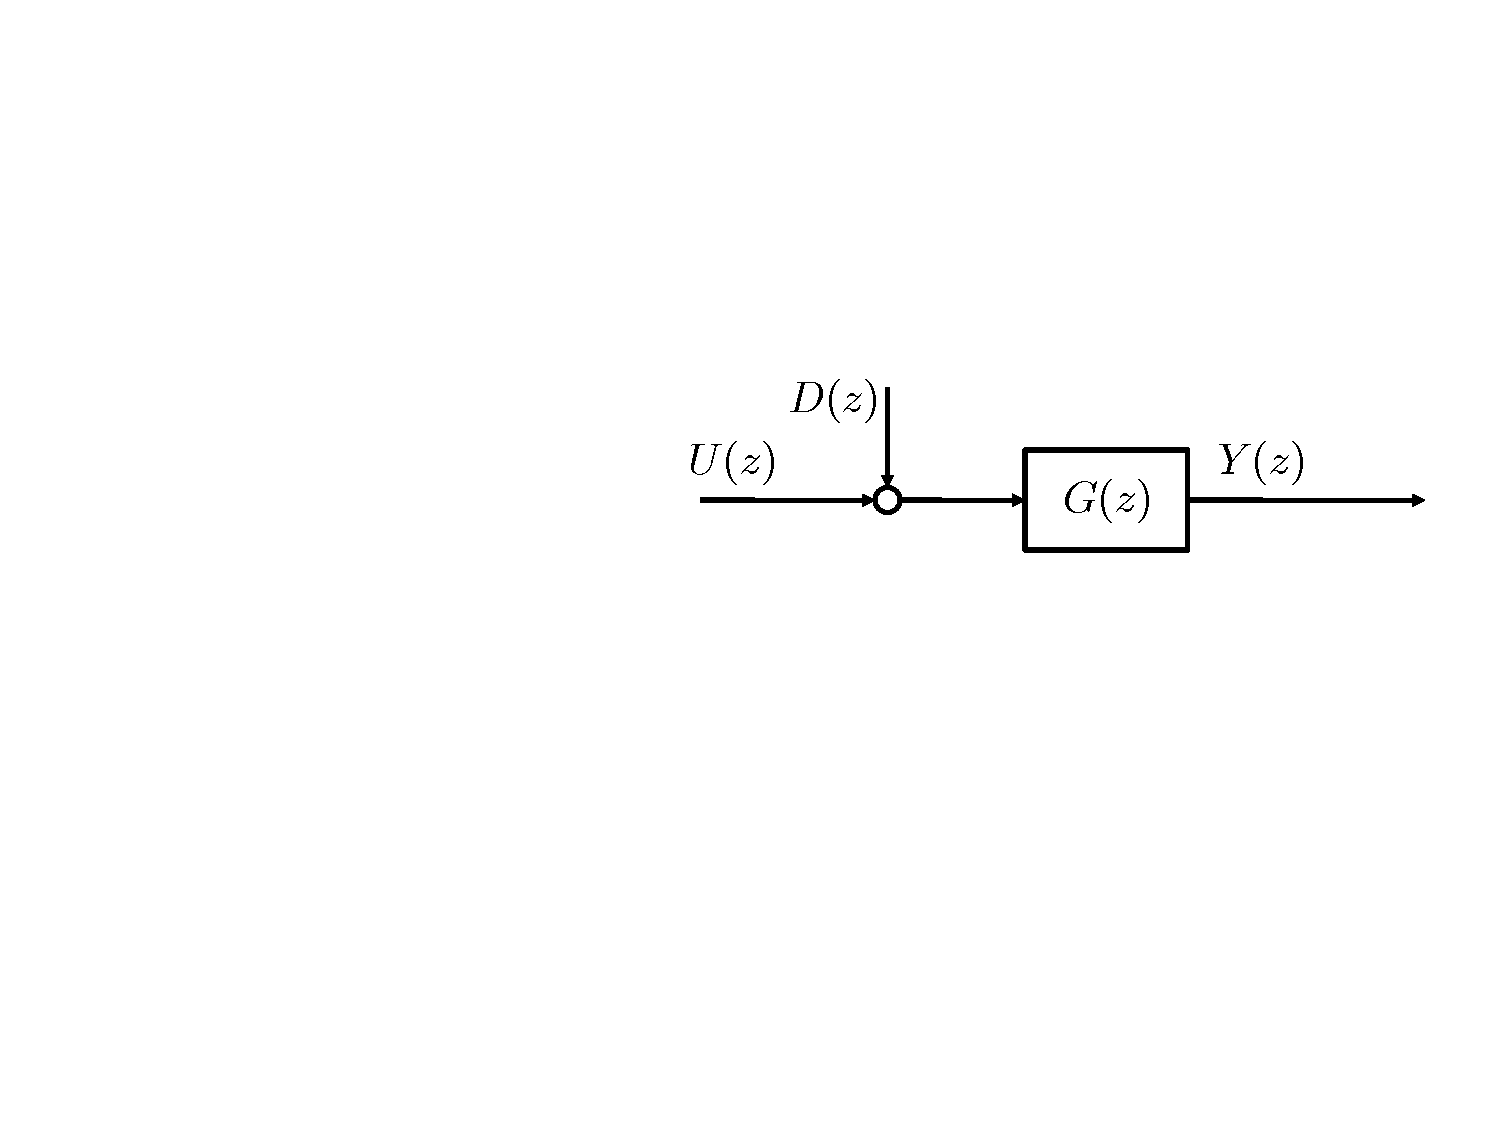
\includegraphics[width=0.5\textwidth]{Disturbance_Observer_motiv1}\\
    \end{figure}

    The signals are:

    \begin{center}
    \begin{tabular}{l @{ : } l}
        $U(z)$ & control input \\
        $D(z)$ & disturbance \\
        $Y(z)$ & output
    \end{tabular}
    \end{center}
    \pause

    The goal is to cancel the effect of $D(z)$ on $Y(z)$
\end{frame}

\begin{frame}
    \frametitle{Motivation}
    \begin{itemize}
    \item
    Let the plant be given by the transfer function $G_n(z)$, which is \underline{minimum phase} (i.e.\ its poles and zeros are strictly inside the unit disk in the complex plane)
    \pause

    \item
    Use an inverse plant to reconstruct $U(z) + D(z)$:
    \begin{figure}
        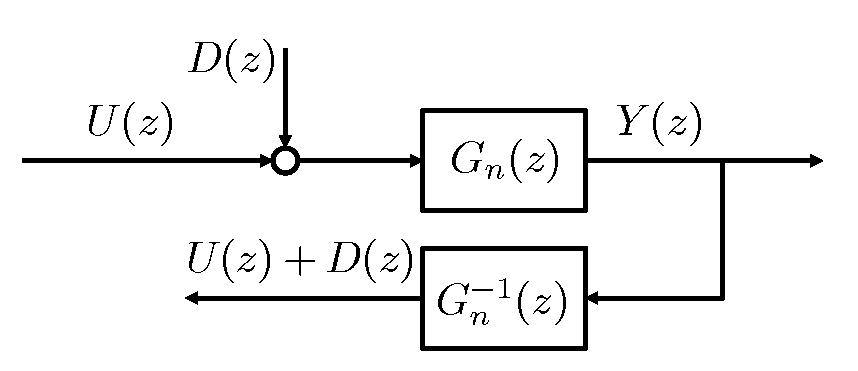
\includegraphics[width=0.5\textwidth]{Disturbance_Observer_motiv2}\\
    \end{figure}
    \pause

    \item
    Subtract $U(z)$ to reconstruct $D(z)$:
    \begin{figure}
        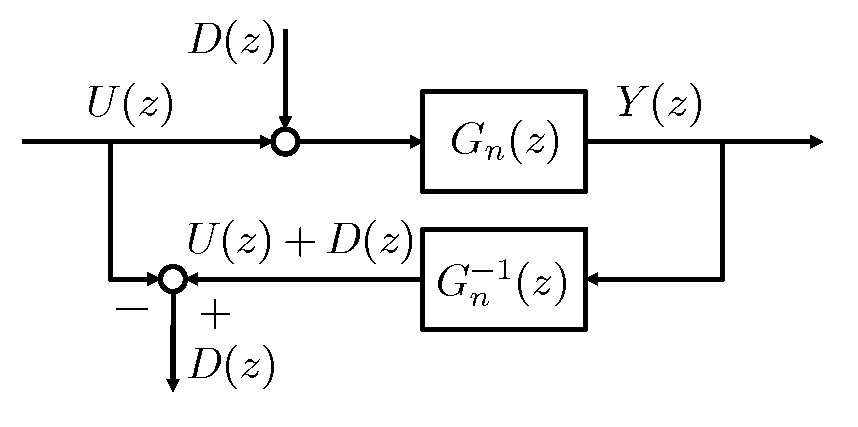
\includegraphics[width=0.5\textwidth]{Disturbance_Observer_motiv3}\\
    \end{figure}

    \end{itemize}
\end{frame}

\begin{frame}
    \frametitle{Motivation}
    \begin{itemize}
    \item
    Ideally, we would subtract the reconstructed value of $D(z)$ from $U(z)$
    \begin{figure}
        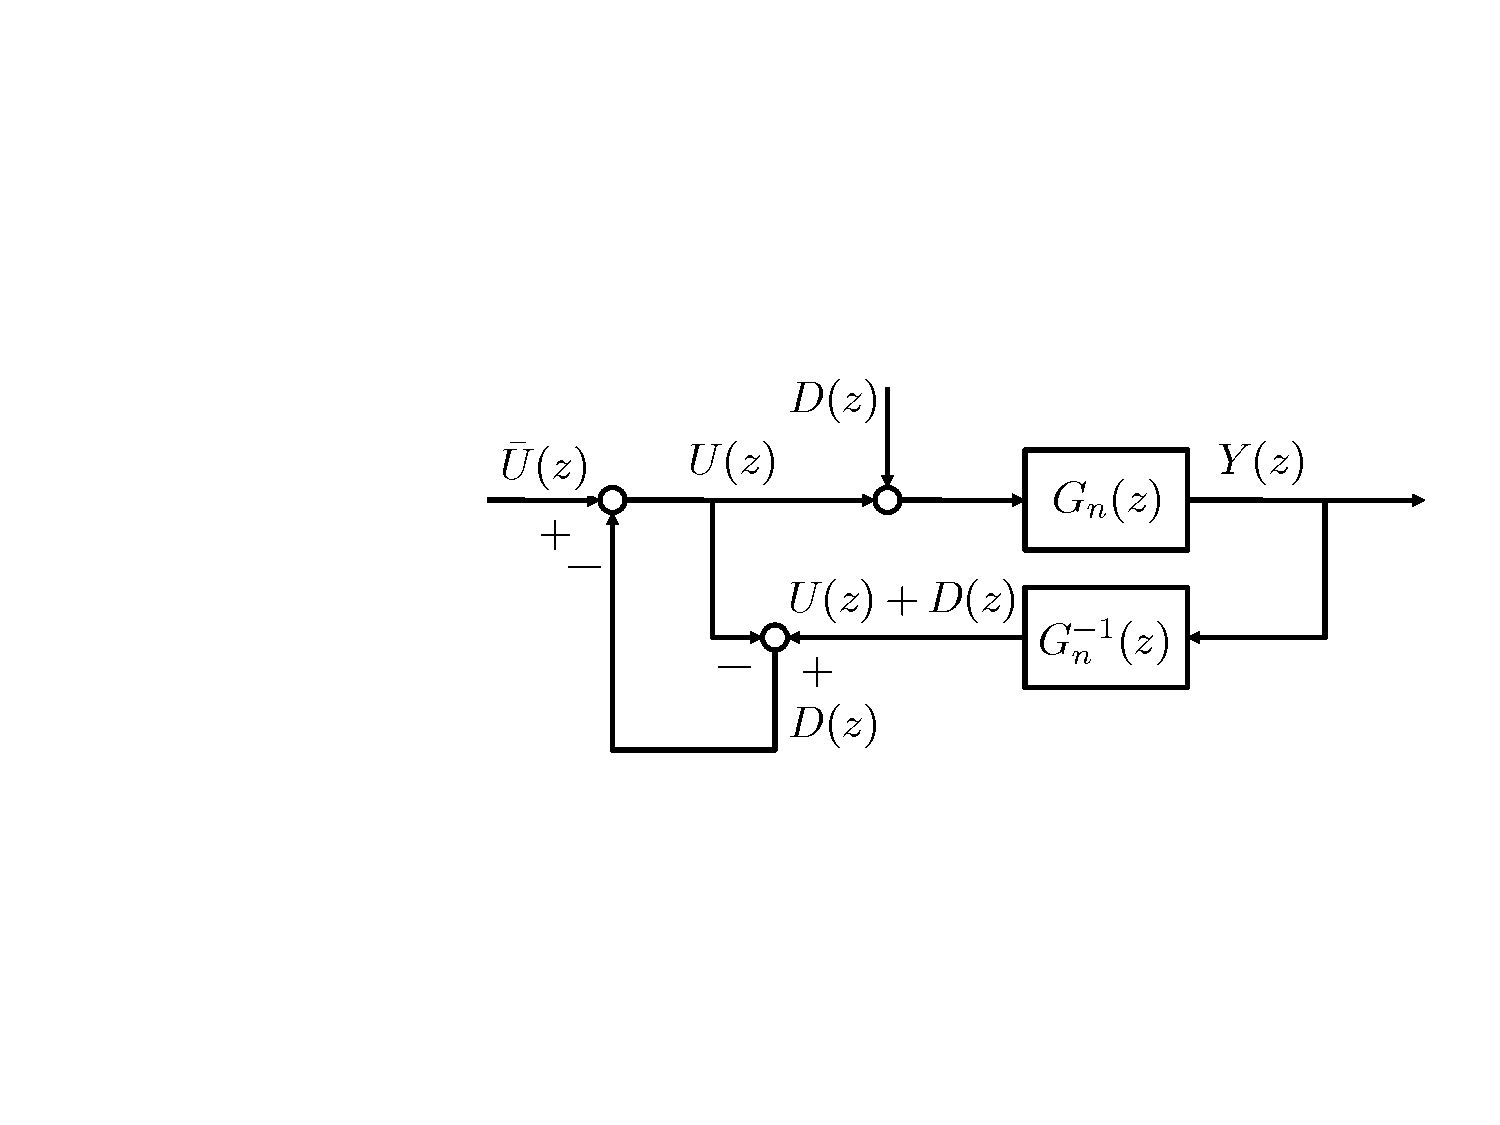
\includegraphics[width=0.7\textwidth]{Disturbance_Observer_motiv4}\\
    \end{figure}
    \pause

    \item
    This would yield the closed-loop dynamics $Y(z) = G_n(z) \bar{U}(z)$
    \end{itemize}
    \pause


    This controller structure would reconstruct $D(z)$ then subtract it from $U(z)$ so that the effect of the disturbance is \underline{exactly canceled}
    \pause

    $\Rightarrow$ This would be useful as an inner loop of a larger control scheme, \underline{BUT...}

\end{frame}

\begin{frame}
    \frametitle{Motivation---Problems}
    \begin{figure}
        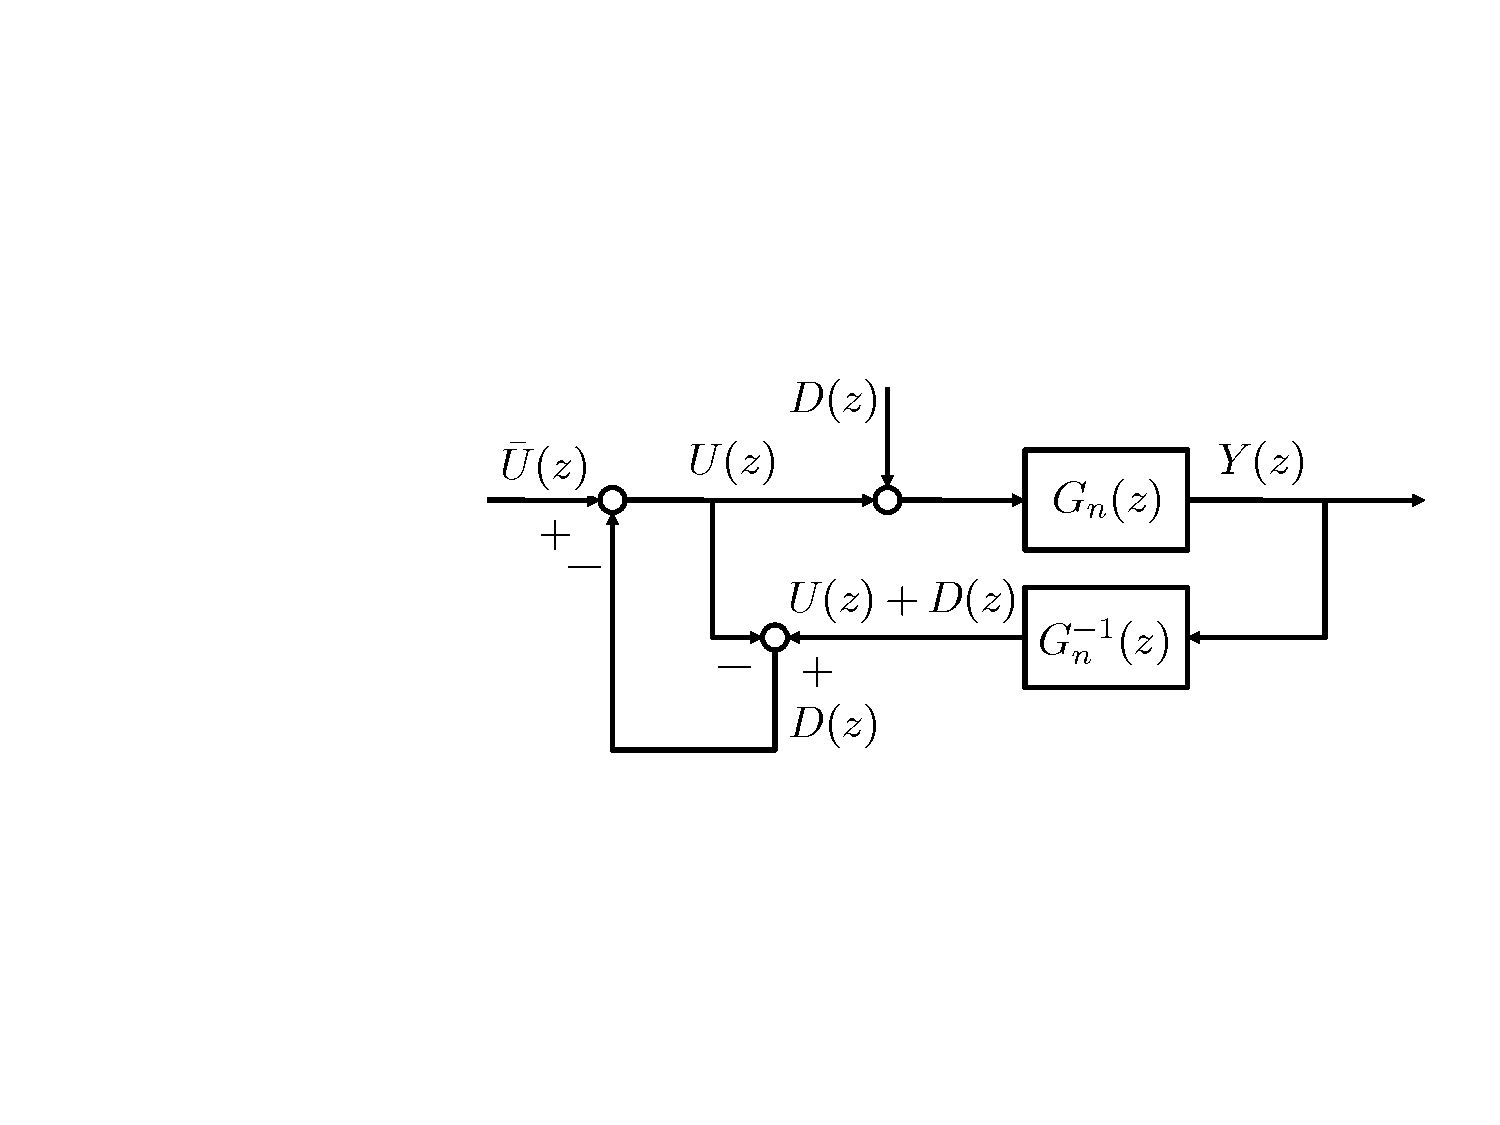
\includegraphics[width=0.5\textwidth]{Disturbance_Observer_motiv4}\\
    \end{figure}

    The control structure has some problems that should be resolved in order for it to be useful:

    \begin{itemize}
    \item
    Since $G_n^{-1}(z)$ is typically not proper, it is not realizable
    \pause

    $\Rightarrow$ We cannot reconstruct $D(z)$
    \pause

    \item
    The system being controlled might not be exactly as given by the model $G_n(z)$
    \pause

    \item
    Sensor noise will corrupt the reconstructed value of $D(z)$
    \pause
    
    \item
    The block diagram above is not well-posed and, in particular, $U(z)$ is not a realizable function of $Y(z)$.

    \end{itemize}
\end{frame}


